\documentclass[a4paper,12pt]{scrreprt}
\usepackage[ngerman]{babel}
\usepackage[a4paper]{geometry}
\usepackage{amsmath}
\usepackage{acronym}
\usepackage{graphicx}
\usepackage[onehalfspacing]{setspace}
\usepackage[colorlinks=true, allcolors=blue]{hyperref}
\newcommand{\dcplace}{Aachen}
\newcommand{\dcdate}{04. Mai 2025}
\newcommand{\dcauthorfirstname}{Max}
\newcommand{\dcauthorlastname}{Mustermann}


\begin{document}
\begin{titlepage}
	%ab hier kleinere Raender, mehr bedruckbare Flaeche.
	\thispagestyle{empty}
	\newgeometry{a4paper, portrait, left=1.0cm, right=0cm, top=0.6cm, bottom=0cm, includefoot}

    \noindent
    \begin{minipage}[t]{0.5\textwidth}
        
\includegraphics[width=3.7cm]{firmenlogo.jpg}
    \end{minipage}%
    \begin{minipage}[t]{0.5\textwidth}
          \raggedleft
          
\includegraphics[width=1.7cm]{FHAC.jpg}
    \end{minipage}

	\vspace{1.0cm}

	% Kopfzeile mit Fachbereich ...
	{\centering \bfseries \Large FH~Aachen \\
	\vspace{1cm}
	\normalsize Fachbereich\\
	Elektrotechnik und Informationstechnik \\
	Studiengang~Informatik \par}

	\vspace{1cm}
    
	{\centering \bfseries \large Bachelorarbeit \par}

	\vspace{1cm}

	\centering \begin{minipage}[t]{13cm}
		\centering \small Konzeption und prototypische Entwicklung einer webbasierten Applikation zur Ausschöpfung und Bereistellung von Geodaten \\
        (Data-Konnector für Geodaten)
		\medskip
	\end{minipage}

	\vspace{1.5cm}
    
	%\vspace*{1cm}
	%\hspace*{6.8cm}
	\begin{minipage}[t]{9cm}
		\centering Tuan Anh Cong Nguyen \\ Matr.-Nr.: 3517392
	\end{minipage}
	\vspace{2.1cm}
    
	%\vspace*{4.7cm}
	%\hspace*{6.8cm}
	\centering \begin{minipage}[b]{15cm}
		\centering
			Referent: Prof. Dr. rer. nat. Heinrich Faßbender\\
			%Korreferent: Prof. Dr.-Ing. ...\
	\end{minipage}


	\vspace{1.5cm}
	
	%Erstellungsdatum
	%\vspace{-4cm}
	%\begin{flushright}
	\centering %\hspace{8cm}
	\begin{minipage}[b]{10cm}
			\centering
            In Zusammenarbeit mit Ausbildungsbetrieb:\\
            ahu GmbH Wasser Boden Geomatik \\
            \vspace{1cm}
            Externer Betreuer: Dr. David Loibl
            
			%\today\\ %Datum\\
			%\vspace{1cm}
			%vertraulich bis xx.xx.xx
	\end{minipage}
	%\end{flushright}

	%\today
	\restoregeometry
\end{titlepage}

\clearpage % Neue Seite für Selbstständigkeitserklärung
\chapter*{Selbstständigkeitserklärung}
\thispagestyle{empty}	%keine Seitenzahl!
\pdfbookmark{Selbstständigkeitserklärung}{Selbstständigkeitserklärung}
Ich versichere hiermit, dass ich die vorliegende Arbeit selbständig verfasst und keine anderen als die im Literaturverzeichnis angegebenen Quellen benutzt habe.\\ \\
Stellen, die wörtlich oder sinngemäß aus veröffentlichten oder noch nicht veröffentlichten Quellen entnommen sind, sind als solche kenntlich gemacht.\\ \\ Die Zeichnungen oder Abbildungen in dieser Arbeit sind von mir selbst erstellt worden oder mit einem entsprechenden Quellennachweis versehen.\\ \\ Diese Arbeit ist in gleicher oder ähnlicher Form noch bei keiner anderen Prüfungsbehörde eingereicht worden.\\ \\[2ex]
Aachen, den \today \hspace{4cm} \dotfill 
\tableofcontents

\clearpage
\chapter*{Abkürzungsverzeichnis}\label{abkuerzungsverzeichnis}
\begin{acronym}[YTM]
\setlength{\itemsep}{-\parsep}

\acro{gravitation}[$g$]{\hspace{1cm}Gravitation in Nähe der Erdoberfläche}
\acro{Nu}[$Nu$]{\hspace{1cm}Nußelt-Zahl}
\acro{nu_luft}[$\nu_{Luft}$]{\hspace{1cm}Kinematische Viskosität von Luft}
\acro{Pr}[$Pr$]{\hspace{1cm}Prandtl-Zahl}
\acro{Q}[$\dot Q$]{\hspace{1cm}Wärmestrom}
\acro{Ra}[$Ra$]{\hspace{1cm}Rayleigh-Zahl}
\acro{rho_luft}[$\rho_{Luft}$]{\hspace{1cm}Dichte von Luft}
\acro{temperatur}[$T$]{\hspace{1cm}Temperatur}
\acro{umgebungstemperatur}[$T_{\infty}$]{\hspace{1cm}Umgebungstemperatur}

\end{acronym}

\cleardoublepage
\chapter*{Abstract}
\thispagestyle{plain}
\addcontentsline{toc}{chapter}{Abstract}
In einer zunehmend digitalisierten und automatisierten Welt wächst täglich die Menge an neu generierten Geodaten – insbesondere Mess- und räumlichen Daten.\\ \\
Die Suche nach und Einbindung von OGC-Geodatendiensten wie WMS (Web Map Service) und WFS (Web Feature Service) in Geoinformationssysteme wie QGIS kann tatsächlich schwierig sein. Die Suche erfordert den Anwender oft das Durchforsten verschiedener Quellen und die manuelle Überpüfung von Dienstbeschreibung. Eine automatisiert und effiziente Lösung kann teilweise helfen, diesen Prozess zu verbessern. \\ 
Die Suche nach Messdaten wie Grundwasserständen, Pegelständen und Klimadaten (Niederschlag,Temperatur) und deren Umformatierung in ein einheitliches Format gestalten sich als schwierig und kompliziert, da es eine Vielzahl von Datenanbietern mit unterschiedliche Datenstrukturen, Formen, etc. gibt.\\ \\
Die Bereitstellung dieser Rohdaten erfolgt meinst im CSV-Format oder als individuell strukturtierte ASCII-Dateien. Im Kontext von der Datenkonsum, gibt es bei der Ahu den sogenannten ahuManager-Client, der diese Daten konsumiert. Bevor diese konsumieren können, müssen die Rohdaten in ein kompatibeles Format umformatiert werden, was bisher teilweise von Hand erledigt werden (in Excel o.ä.). Diese manuelle Vorgehen kann perspektivisch zum Teil oder ganz automatisiert werden, was die Produktivität steigert und die Fehleranfälligkeit vermeidet. \\ \\
Daher befasst sich diese Arbeit  mit dem Thema, wie eine webbasierte Applikation zur Ausschöpfung und Bereitstellung von rohen Geodaten im Kontext von der Abteilung Geomatik von Ahu GmbH entwickelt werden kann.

\clearpage
\chapter{Einleitung}

\section{Motivation der Arbeit}


\section{Ziel der Arbeit}


\chapter{Some examples to get started}
\section{How to create Sections and Subsections}

\section{How to include Figures}
Note that your figure will automatically be placed in the most appropriate place for it, given the surrounding text and taking into account other figures or tables that may be close by. You can find out more about adding images to your documents in this help article on \href{https://www.overleaf.com/learn/how-to/Including_images_on_Overleaf}{including images on Overleaf}.
\subsection{How to add Tables}

\begin{figure}
\centering
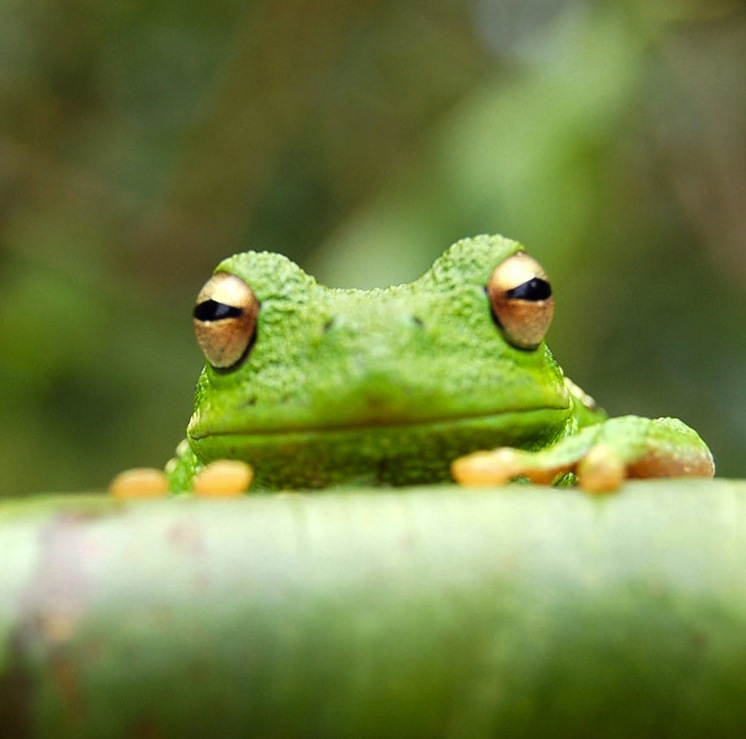
\includegraphics[width=0.25\linewidth]{frog.jpg}
\caption{\label{fig:frog}This frog was uploaded via the file-tree menu.}
\end{figure}


Use the table and tabular environments for basic tables --- see Table~\ref{tab:widgets}, for example. For more information, please see this help article on \href{https://www.overleaf.com/learn/latex/tables}{tables}. 

\begin{table}
\centering
\begin{tabular}{l|r}
Item & Quantity \\\hline
Widgets & 42 \\
Gadgets & 13
\end{tabular}
\caption{\label{tab:widgets}An example table.}
\end{table}

\section{How to add Comments and Track Changes}

Track changes are available on all our \href{https://www.overleaf.com/user/subscription/plans}{premium plans}, and can be toggled on or off using the option at the top of the Review pane. Track changes allow you to keep track of every change made to the document, along with the person making the change. 

\section{How to add Lists}

You can make lists with automatic numbering \dots

\begin{enumerate}
\item Like this,
\item and like this.
\end{enumerate}
\dots or bullet points \dots
\begin{itemize}
\item Like this,
\item and like this.
\end{itemize}

\section{How to write Mathematics}

\LaTeX{} is great at typesetting mathematics. Let $X_1, X_2, \ldots, X_n$ be a sequence of independent and identically distributed random variables with $\text{E}[X_i] = \mu$ and $\text{Var}[X_i] = \sigma^2 < \infty$, and let
\[S_n = \frac{X_1 + X_2 + \cdots + X_n}{n}
      = \frac{1}{n}\sum_{i}^{n} X_i\]
denote their mean. Then as $n$ approaches infinity, the random variables $\sqrt{n}(S_n - \mu)$ converge in distribution to a normal $\mathcal{N}(0, \sigma^2)$.


\section{How to change the margins and paper size}

Usually the template you're using will have the page margins and paper size set correctly for that use-case. For example, if you're using a journal article template provided by the journal publisher, that template will be formatted according to their requirements. In these cases, it's best not to alter the margins directly.

If however you're using a more general template, such as this one, and would like to alter the margins, a common way to do so is via the geometry package. You can find the geometry package loaded in the preamble at the top of this example file, and if you'd like to learn more about how to adjust the settings, please visit this help article on \href{https://www.overleaf.com/learn/latex/page_size_and_margins}{page size and margins}.

\section{How to change the document language and spell check settings}

Overleaf supports many different languages, including multiple different languages within one document. 

To configure the document language, simply edit the option provided to the babel package in the preamble at the top of this example project. To learn more about the different options, please visit this help article on \href{https://www.overleaf.com/learn/latex/International_language_support}{international language support}.

To change the spell check language, simply open the Overleaf menu at the top left of the editor window, scroll down to the spell check setting, and adjust accordingly.

\section{How to add Citations and a References List}

You can simply upload a \verb|.bib| file containing your BibTeX entries, created with a tool such as JabRef. You can then cite entries from it, like this: \cite{greenwade93}. Just remember to specify a bibliography style, as well as the filename of the \verb|.bib|. You can find a \href{https://www.overleaf.com/help/97-how-to-include-a-bibliography-using-bibtex}{video tutorial here} to learn more about BibTeX.

If you have an \href{https://www.overleaf.com/user/subscription/plans}{upgraded account}, you can also import your Mendeley or Zotero library directly as a \verb|.bib| file, via the upload menu in the file-tree.

\section{Good luck!}

We hope you find Overleaf useful, and do take a look at our \href{https://www.overleaf.com/learn}{help library} for more tutorials and user guides! Please also let us know if you have any feedback using the Contact Us link at the bottom of the Overleaf menu --- or use the contact form at \url{https://www.overleaf.com/contact}.

\bibliographystyle{alpha}
\bibliography{sample}

\end{document}